\documentclass[journal=jcisd8,manuscript=article]{achemso}

\usepackage{amsmath}
\usepackage{amssymb}
\usepackage{booktabs}
\usepackage{graphicx}
\usepackage{xcolor}
\usepackage{microtype}

\author{Polina Vinogradova}
\affiliation{Input Output Global, Singapore}
\altaffiliation{ORCID: 0000-0003-3271-3841}
\email{polina.vinogradova@iohk.io}

\title{Definitional Instability in Kinase Inhibitor Selectivity:
  An Empirical Characterization Across Four Datasets and Required Properties
  for a Well-Formed Measure}

\abbreviations{S-score, CATDS, pKd, FAERS}
\keywords{kinase inhibitor selectivity, selectivity metrics, binding affinity,
  axiomatic analysis, drug discovery, cheminformatics}

\begin{document}

\noindent\textbf{Polina Vinogradova}\\
Input Output Global, Singapore\\
Email: polina.vinogradova@iohk.io \quad ORCID: 0000-0003-3271-3841

\bigskip
\noindent\textbf{Keywords:} kinase inhibitor selectivity, selectivity metrics,
binding affinity, axiomatic analysis, drug discovery, cheminformatics

\bigskip


\begin{abstract}
Kinase inhibitor selectivity is quantified using several competing definitions
--- S-score, selectivity entropy, Gini coefficient, and ratio-based measures ---
applied interchangeably without justification.
Across four profiling datasets spanning three assay technologies (Davis,
Klaeger, Anastassiadis, and Metz; 68--704 compounds each), we show these
definitions cluster into two families measuring fundamentally different
properties (cross-family $r = 0.14$--$0.62$) and that rank instability is
predictable from binding profile shape.
Three instability sources are identified: definitional noise below the detection
threshold, ratio-specific instability from near-tied top targets, and
distribution-ratio disagreement for promiscuous compounds with a dominant target.
Ratio-based rankings are unreliable at any practically used panel size;
entropy-based rankings stabilize at approximately 110 kinases.
We derive four required properties that any well-formed selectivity measure
should satisfy; no existing definition satisfies all four simultaneously.
\end{abstract}

\section{Introduction}
\label{sec:intro}

Kinase inhibitors are among the most intensely investigated compound classes
in drug discovery, with over 80 FDA-approved agents and several hundred in
clinical development.\cite{Roskoski2024}
Because the human kinome comprises more than 500 proteins sharing a
highly conserved ATP-binding site,\cite{Manning2002} the design of inhibitors
with controlled target profiles remains a central challenge.
Selectivity --- the degree to which a compound's binding activity is
concentrated on intended rather than off-target kinases --- is a primary
criterion in lead optimization and a key determinant of the therapeutic window
of approved drugs.\cite{Bhullar2018}

Despite its importance, selectivity is not formally defined.
The field employs at least four distinct quantitative measures:
the S-score,\cite{Karaman2008} selectivity entropy,\cite{Uitdehaag2011}
Gini coefficient,\cite{Graczyk2010} and ratio-based measures including the
CATDS score.\cite{Klaeger2017}
These definitions are applied interchangeably in the literature without
systematic justification, and their parameter values --- the activity threshold
in the S-score, the baseline in the entropy and Gini coefficient, the reference
off-target in ratio-based measures --- are chosen by convention rather than
principle.
Standardizing them is a prerequisite for integrating selectivity data across
laboratories and platforms.

Bosc et al.\cite{Bosc2017} showed that these definitions can produce
substantially different compound rankings on the same dataset, and the
KInhibition platform\cite{KInhibition2018} explicitly acknowledged that
conflicting results across metrics are common.
However, the structural sources of this disagreement --- which binding profile
properties determine when definitions agree or conflict, and why --- have not
been characterized.

The absence of a principled basis for selectivity measurement is not merely
a practical inconvenience.
Go/no-go decisions worth hundreds of millions of dollars in development costs
are made on the basis of selectivity assessments whose sensitivity to
definitional choice is unknown.
When a compound is described as ``selective'' in the literature, the claim is
implicitly conditioned on a specific definition and parameterization that is
rarely stated explicitly and almost never justified.
This situation is analogous to measuring temperature with instruments whose
scales have not been calibrated to a common reference: the measurements are
internally consistent but not directly comparable.

Counterintuitively, we find that the compounds most resistant to
definitional disagreement are not the most selective but the most promiscuous:
compounds that bind nearly the entire profiled kinome receive consistent
rankings regardless of which definition is applied, because all definitions
agree they are non-selective.
It is compounds at intermediate promiscuity --- those with one dominant target
and several moderate off-targets, or those with near-identical affinities for
their top two targets --- that receive contradictory rankings depending on
which definition is chosen.
This observation points to a deeper problem: the definitions are not merely
different operationalizations of the same concept, but answers to genuinely
different questions about binding profiles.

This suggests a way forward that has worked in other fields where several
competing measures coexisted.
In information theory, Shannon\cite{Shannon1948} settled which function should
measure uncertainty by writing down a few properties a sensible measure must
have (for example, that it should be maximal when all outcomes are equally
likely) and showing that only entropy satisfies them.
The first step in that approach is always the same: characterize how the
competing measures actually behave, then state the properties a good measure
should have.

This paper takes that first step for kinase inhibitor selectivity, using four
large profiling datasets that span three assay technologies.
Its contributions are as follows.
First, we show that existing definitions cluster into two families ---
distribution-based (S-score, entropy, Gini) and ratio-based (CATDS and
variants) --- that correlate weakly with one another across all four datasets
(cross-family $r = 0.14$--$0.62$) and measure fundamentally different
properties of binding profiles.
Second, we identify three sources of instability: definitional noise for
compounds below the assay detection threshold, ratio-specific instability
driven by near-tied top targets, and distribution-ratio disagreement for
compounds with one dominant target and broad moderate off-target activity.
Third, we propose four required properties --- a reliability threshold condition,
bounded gap sensitivity, distributional consistency, and monotonicity under
weak off-target addition --- and show that no existing definition satisfies
all four simultaneously.
\section{Related Work}
\label{sec:related}

\subsection{Existing Selectivity Metrics and Their Comparison}
\label{sec:related:metrics}

Several metrics have been proposed to quantify kinase inhibitor selectivity
from profiling panel data.
Karaman et al.\cite{Karaman2008} introduced the selectivity score (S-score),
defined as the fraction of panel kinases inhibited above a fixed concentration
threshold.
Uitdehaag and Zaman\cite{Uitdehaag2011} proposed the selectivity entropy,
which treats the normalized binding profile as a probability distribution and
computes its Shannon entropy; low entropy indicates activity concentrated on
few targets.
Graczyk\cite{Graczyk2010} adapted the Gini coefficient from economics, treating
the distribution of a compound's activity across the panel as an inequality
distribution; a value near 1 indicates activity concentrated on few kinases and
near 0 indicates activity spread evenly.
Klaeger et al.\cite{Klaeger2017} introduced the concentration- and
target-dependent selectivity (CATDS) score, which quantifies the reduction in
binding to a given target relative to the summed reduction across all detected
targets at a specified inhibitor concentration.
Bosc et al.\cite{Bosc2017} subsequently proposed two further metrics ---
the window score and ranking score --- and performed a comparative analysis of
all five definitions on the Davis and Anastassiadis datasets, showing that
compound rankings differ substantially depending on the metric applied and that
certain compounds cannot be scored under some definitions when threshold
conditions are not satisfied.

Reconciliation attempts have remained limited in scope.
Bajorath et al.\cite{Bajorath2018} compared CATDS-based selectivity
assessments from Klaeger et al.\ with activity data mined from ChEMBL for the
same compounds, finding broad consistency between the two sources but noting
that no simple relationship between selectivity and clinical performance was
apparent.
The KInhibition platform\cite{KInhibition2018} explicitly acknowledged that
multiple metrics yield conflicting results for the same compound but addressed
this through a unified query interface rather than theoretical analysis.

A common limitation of these studies is that each metric is evaluated at fixed
parameter values, so the sensitivity of rankings to parameter choice has not
been systematically characterized.
The structural properties of binding profiles that determine when definitions
agree or disagree have not been identified.
The present work addresses both gaps.

\subsection{Axiomatic Approaches to Ranking and Measurement}
\label{sec:related:axiomatic}

Axiomatic characterization of measurement functions is well-established in
adjacent fields.
Shannon\cite{Shannon1948} demonstrated that the entropy of a probability
distribution is uniquely determined, up to a multiplicative constant, by four
requirements: continuity, maximality on the uniform distribution,
expansibility, and additivity over independent subsystems.
Khinchin\cite{Khinchin1957} subsequently strengthened this uniqueness result.
The selectivity entropy of Uitdehaag and Zaman applies the Shannon formula to
normalized binding profiles but provides no analogous axiomatic justification;
it is not known whether it is the unique function satisfying reasonable
selectivity-specific properties, or one of many equivalent alternatives.

Arrow\cite{Arrow1951} established that no social welfare function satisfies
simultaneously the requirements of unrestricted domain, Pareto efficiency,
independence of irrelevant alternatives, and non-dictatorship.
The theorem is relevant here in two respects: it demonstrates that axiomatic
analysis of a ranking concept can yield impossibility rather than uniqueness,
and it shows that competing ranking functions reflect genuine tradeoffs between
properties that cannot all be achieved simultaneously.
Singleton and Booth\cite{Singleton2022} applied this methodology to truth
discovery --- the problem of identifying true facts from conflicting reports of
unknown reliability --- posing it as a social choice problem, formulating
candidate axioms, and proving that a subset cannot be jointly satisfied.
The structure of that problem is closely analogous to selectivity measurement,
where multiple definitions produce conflicting rankings and the question of
which to trust is unresolved.

To our knowledge, this axiomatic style of analysis has not previously been
applied to any selectivity or promiscuity measure in drug discovery.
The present work proposes empirically motivated required properties as a
foundation for such an analysis.

\section{Methods}
\label{sec:methods}

\subsection{Datasets}
\label{sec:methods:data}

Two publicly available kinase inhibitor profiling datasets were used.
The Davis dataset\cite{Davis2011} comprises binding affinities ($K_d$) for 68
small-molecule kinase inhibitors measured against 433 human kinase domains.
Affinity values are reported as dissociation constants and were converted to
$\mathrm{p}K_d = -\log_{10}(K_d / 10^9)$ prior to analysis, following the
convention of the DeepDTA benchmark.\cite{DeepDTA}
Pairs for which no binding was detected at the screening concentration of
10~$\mu$M were assigned $\mathrm{p}K_d = 5.0$, corresponding to a $K_d$ of
1~mM, which represents the detection floor of the assay.
The resulting affinity matrix is complete ($68 \times 433$, 29{,}444 entries),
with all non-binding pairs assigned the detection-floor value
$\mathrm{p}K_d = 5.0$.
This is the standard convention for the dataset\cite{DeepDTA,Bosc2017} and
slightly underestimates true non-binding affinity.

The Klaeger dataset\cite{Klaeger2017} comprises binding affinities for 243
clinical kinase inhibitors profiled against the human kinome using
Kinobeads chemical proteomics.
Apparent dissociation constants ($K_d^\mathrm{app}$) were derived from
dose--response curves across eight inhibitor concentrations in cancer cell
lysates.
Only high-confidence measurements (as annotated by the original authors) were
retained, yielding 5{,}123 drug--target pairs for 222 drugs and 343 kinase
targets.
Affinity values were converted to $\mathrm{p}K_d$ using the same formula as
above.
Missing entries, representing kinase--inhibitor combinations not detected in
the assay, were assigned the background value $\mathrm{p}K_d = 5.0$.
The resulting Klaeger matrix is $222 \times 343$.
The fraction of active entries (pKd $> 6$, i.e.\ $K_d < 1~\mu$M) is 17.9\% for
Davis and 3.6\% for Klaeger, reflecting the more stringent detection threshold
of the chemoproteomic assay.

To test whether our findings depend on the assay technology, we added two
further datasets that measure kinase inhibition by different means.
The Anastassiadis dataset\cite{Anastassiadis2011} profiles 178 inhibitors
against 300 kinases in a single-concentration ($0.5~\mu$M) radiometric activity
assay, reported as percent residual kinase activity relative to a solvent
control.
We converted these to percent inhibition ($100$ minus residual activity,
clipped to $[0,100]$; higher values denote stronger inhibition), with the
$1.1\%$ missing entries set to zero inhibition.
The Metz dataset\cite{Metz2011} reports $\mathrm{p}K_i$ affinities --- the same
negative-log scale as $\mathrm{p}K_d$ --- for a large medicinal-chemistry
campaign; we restricted it to the 704 compounds profiled against at least 50 of
the 172 kinases, assigning the assay floor $\mathrm{p}K_i = 4.0$ to unmeasured
combinations.
The four datasets thus span three assay technologies (competition binding,
chemoproteomics, and functional activity) and two readout types (affinity and
single-concentration inhibition).
Because each selectivity definition is computed on the native readout of its
dataset and our analyses concern rank correlations between definitions and rank
instability --- both invariant to a common monotone rescaling within a dataset
--- the definitions remain directly comparable across datasets.
For the percent-inhibition and $\mathrm{p}K_i$ datasets the parameter sweeps
were shifted to the corresponding scale (S-score thresholds and entropy/Gini
baselines spanning each dataset's active range; reference off-targets
$k \in \{1,\ldots,5\}$ as before).

We did not include two further datasets named by a reviewer.
The Gao screen\cite{Gao2013} is a single-concentration functional inhibition
assay of the same readout type as the Anastassiadis dataset already included,
and its raw data are not openly redistributable; including it would add a
second instance of an assay type rather than a new modality.
The Patricelli study\cite{Patricelli2011} profiles only a small number of
inhibitors against native kinases as a proof of concept for the KiNativ
platform; a ranking-stability analysis requires many compounds to produce a
meaningful ranking, so this dataset is not suited to the present comparison.

\subsection{Selectivity Definitions and Parameterization}
\label{sec:methods:defs}

Four selectivity definitions were implemented, each controlled by one or more
parameters whose values are not standardized in the literature.
For each definition we state below the quantity defined in the original
publication, the form in which we implemented it, and a plain-language
description of what it measures.
Throughout, a compound's binding profile is the vector of its affinities
$\mathrm{p}K_{d,i}$ across the $N$ panel kinases, with higher
$\mathrm{p}K_{d}$ denoting tighter binding.

\paragraph{S-score.}
Karaman et al.\cite{Karaman2008} defined the selectivity score as the fraction
of the panel that a compound inhibits: the number of kinases ``bound'' divided
by the number tested, where a kinase counts as bound when the compound reduces
its activity below a fixed cutoff at a single screening concentration (the
original work reports $S(35)$, $S(10)$ and $S(1)$ for cutoffs of $35\%$, $10\%$
and $1\%$ of control activity).
We implemented the same fraction, expressing the bound criterion as an affinity
threshold $\tau$ on $\mathrm{p}K_d$:
\begin{equation}
  S(\tau) = \frac{1}{N} \sum_{i=1}^{N} \mathbf{1}[\mathrm{p}K_{d,i} > \tau].
\end{equation}
Sweeping $\tau$ reproduces Karaman's family of cutoffs; we used
$\tau \in \{5.5, 5.75, \ldots, 8.0\}$ (11 values), spanning $K_d$ cutoffs from
approximately 300~nM to 10~nM.
\emph{In words:} what fraction of all tested kinases does the compound
appreciably hit? A smaller fraction means greater selectivity.

\paragraph{Selectivity entropy.}
Uitdehaag and Zaman\cite{Uitdehaag2011} treat the compound's binding across the
panel as a probability distribution and report its Shannon entropy; a profile
concentrated on few kinases has low entropy and is selective.
In the original definition the weight on each kinase is its association constant
$K_{a,i} = 1/K_{d,i}$ (the share of compound that would be bound to kinase $i$
in an equimolar mixture), so $p_i = K_{a,i}/\sum_j K_{a,j}$.
We implemented the entropy on the same log-affinity scale used by the other
metrics, weighting each kinase by its affinity in excess of a baseline $\beta$:
\begin{equation}
  H(\beta) = -\sum_{i=1}^{N} p_i \log_2 p_i, \quad
  p_i = \frac{\max(\mathrm{p}K_{d,i} - \beta,\, 0)}
             {\sum_j \max(\mathrm{p}K_{d,j} - \beta,\, 0)},
\end{equation}
where $\beta$ is the affinity below which binding is treated as negligible.
This makes $\beta$ an explicit parameter (its under-specification motivates
property D3 below); we swept $\beta \in \{5.0, 5.25, \ldots, 6.5\}$ (7 values).
The association-constant and log-affinity weightings are distinct reasonable
choices that can rank compounds differently, which is itself an instance of the
definitional instability this paper characterizes; we quantify the difference
below (``Faithfulness to the original definitions'').
Lower entropy indicates greater selectivity.
\emph{In words:} how spread out is the compound's binding across the kinome?
Binding concentrated on few targets gives low entropy and high selectivity.

\paragraph{Gini coefficient.}
Graczyk\cite{Graczyk2010} adapted the Gini coefficient from economics: kinases
are sorted by activity and the cumulative fraction of total binding is plotted
against the cumulative fraction of kinases (a Lorenz curve); the Gini
coefficient is twice the area between this curve and the diagonal of equal
distribution.
The original work computes it from percent-inhibition values.
We applied the standard discrete Gini formula to the same baseline-subtracted
log-affinities used for the entropy:
\begin{equation}
  G(\beta) = \frac{2\sum_{i=1}^{N} i \cdot x_{(i)}}{N \sum_{i=1}^{N} x_{(i)}} - \frac{N+1}{N},
  \qquad x_{(i)} = \max(\mathrm{p}K_{d,i} - \beta,\, 0)\ \text{sorted ascending}.
\end{equation}
We swept $\beta$ over the same range as for the entropy.
A compound whose binding is concentrated on one kinase has a highly unequal
distribution and $G$ near 1; a compound that binds many kinases equally has
$G$ near 0.
Higher values therefore indicate greater selectivity.
\emph{In words:} how unequally is binding distributed across the kinome?
The more unequal, the more selective.

\paragraph{Ratio.}
Classical pharmacological selectivity is pairwise: how much more tightly does a
compound bind its primary target than an off-target?
We implemented this as the fold-selectivity, in log units, between the primary
target and the $k$-th ranked off-target:
\begin{equation}
  R(k) = \mathrm{p}K_{d,(1)} - \mathrm{p}K_{d,(k+1)}
       = \log_{10}\!\frac{K_{d,(k+1)}}{K_{d,(1)}},
\end{equation}
where $\mathrm{p}K_{d,(j)}$ is the $j$-th largest affinity in the profile and
$k \in \{1, 2, 3, 4, 5\}$ selects the reference off-target.
This is the prototypical member of the ratio family, which also includes the
concentration- and target-dependent selectivity (CATDS) score of Klaeger et
al.\cite{Klaeger2017} --- a concentration-dependent fraction quantifying the
binding reduction at one target relative to the summed reduction across all
targets.
We use the simpler fold-selectivity because the reference off-target index $k$
is then an explicit parameter whose effect can be studied directly.
A larger affinity gap to the nearest competitor means greater selectivity, so
higher $R(k)$ indicates greater selectivity.
\emph{In words:} how big is the affinity gap between the primary target and the
next-best one? A larger gap means greater selectivity.

\paragraph{Faithfulness to the original definitions.}
The S-score and the ratio are computed in the form given by their original
sources (a panel-hit fraction and a primary-to-off-target affinity ratio,
respectively).
For the entropy and the Gini coefficient we used the baseline-subtracted
log-affinity profile in place of the original association constants (entropy)
and percent-inhibition values (Gini), so that all four metrics operate on one
common scale and so that the baseline $\beta$ appears as an explicit parameter.
To confirm that this choice does not silently determine our conclusions, we
recomputed the entropy and Gini in forms closer to the originals
(association-constant weighting) and compared the resulting rankings with the
log-affinity forms.
The two operationalizations differ substantially --- for entropy, Spearman
$r = 0.42$ (Davis) and $-0.32$ (Klaeger); for Gini, $r = 0.11$ and $-0.46$
(Supporting Information, Figure~S1) --- confirming that the operationalization
of a named metric is itself a source of the definitional instability we report,
not a neutral implementation detail.

\subsection{Rank Stability Analysis}
\label{sec:methods:stability}

For each definition and each parameter value, compounds were ranked from most
selective (rank 1) to least selective (rank $n$, where $n$ is the number of
compounds in the dataset).
Ties were broken by average rank.
This yielded 30 rank vectors per dataset: 11 for the S-score, 7 for entropy,
7 for Gini, and 5 for ratio.

For each compound, rank instability was quantified as the standard deviation
of its rank across all 30 configurations (overall instability) and separately
across configurations within each definition family (within-family
instability).
Cross-definition agreement was assessed using Spearman rank correlation
between the median rank vectors of each definition family.
The median was taken across parameter values within each family prior to
correlation to obtain a single representative ranking per definition.

Associations between rank instability and binding profile features were
assessed using Spearman correlation.
Profile features computed for each compound included: the number of active
kinases ($\mathrm{p}K_d > 6$), the gap between the top and second-ranked
affinities, the standard deviation and range of active affinities, and the
absolute affinity of the second-ranked target.
All correlations are reported with two-tailed $p$-values; significance
thresholds of $p < 0.05$, $p < 0.01$, and $p < 0.001$ are denoted *, **, and
*** respectively.
Analyses were performed in Python 3.10 using NumPy, pandas, and
SciPy.\cite{NumPy,pandas,SciPy}
A secondary analysis relating selectivity rankings to clinical adverse-event
outcomes (FAERS report rates and FDA-label discontinuation rates for the
FDA-approved Klaeger compounds) is summarized in the Limitations and reported
in full in the Supporting Information.

\section{Results}
\label{sec:results}

\subsection{Selectivity Definitions Cluster into Two Families}
\label{sec:results:families}

Across 30 parameter configurations (11 S-score thresholds, 7 entropy
baselines, 7 Gini baselines, 5 ratio off-target indices), compound rankings
were computed for all drugs in both datasets.
Spearman correlations between the median ranking of each definition family
reveal a consistent two-cluster structure (Table~\ref{tab:correlations}).
On the Davis dataset, S-score, entropy, and Gini are mutually correlated
($r = 0.91$--$0.999$), while ratio correlates substantially less with each
($r = 0.34$--$0.45$).
On the larger Klaeger dataset, the same structure is preserved but with lower
within-cluster correlations ($r = 0.75$--$0.91$), reflecting greater
diversity of binding profiles among the 222 clinical compounds.
The ratio definition is the consistent outlier in both datasets, with
cross-family correlations of $r = 0.27$--$0.62$.

\begin{table}[h]
  \centering
  \caption{Spearman correlations between median rankings by definition family.
           Upper triangle: Davis ($n=68$). Lower triangle: Klaeger ($n=222$).}
  \label{tab:correlations}
  \begin{tabular}{lcccc}
    \toprule
                & S-score & Entropy & Gini  & Ratio \\
    \midrule
    S-score     & ---     & 0.949   & 0.954 & 0.454 \\
    Entropy     & 0.910   & ---     & 0.999 & 0.343 \\
    Gini        & 0.745   & 0.869   & ---   & 0.343 \\
    Ratio       & 0.265   & 0.480   & 0.617 & ---   \\
    \bottomrule
  \end{tabular}
\end{table}

This two-family structure reflects a fundamental difference in what the
definitions measure.
The S-score, entropy, and Gini all quantify the concentration of activity
across the full kinase panel; they differ in functional form but respond to
the same underlying property of the binding profile.
The ratio definition, by contrast, quantifies the gap between the primary
target and a specific off-target, ignoring the remainder of the binding
profile entirely.
A compound that strongly inhibits one kinase and moderately inhibits twenty
others will be ranked as highly selective by ratio (large gap to the
second target) but as moderately promiscuous by entropy and Gini
(activity distributed across many targets).

\subsection{The Two-Family Structure Replicates Across Assay Technologies}
\label{sec:results:replication}

The same two-family structure holds in all four datasets, across three assay
technologies and both readout types (Figure~\ref{fig:crossdataset}).
The S-score, entropy, and Gini remain mutually correlated within each dataset
(within-family Spearman $r = 0.74$--$0.99$), while the ratio definition is the
consistent outlier: its correlation with the distribution-based family is
$r = 0.34$--$0.45$ on Davis, $0.27$--$0.62$ on Klaeger, $0.52$--$0.56$ on the
Anastassiadis functional-activity dataset, and $0.14$--$0.19$ on the Metz
$\mathrm{p}K_i$ dataset.
The degree of separation varies with the assay, but in every case the ratio
definition measures something the distribution-based definitions do not.

The instability findings also replicate.
Compounds with no active kinases (Type~1, below) are markedly more rank-unstable
than active compounds wherever such compounds exist: mean rank
$\sigma = 37.6$ vs.\ $22.0$ on Anastassiadis and $178.7$ vs.\ $108.2$ on Metz,
matching the $73.8$ vs.\ $32.4$ contrast on Klaeger (Davis contains no
zero-active compounds).
Within the distribution-based family, the number of active kinases negatively
predicts entropy instability in every dataset ($r = -0.28$ to $-0.46$), and the
top$_1$--top$_2$ affinity gap predicts ratio instability on Davis, Klaeger, and
Metz ($r = -0.45$, $-0.34$, $-0.26$; all $p < 0.001$), as detailed below.

\begin{figure}[h]
  \centering
  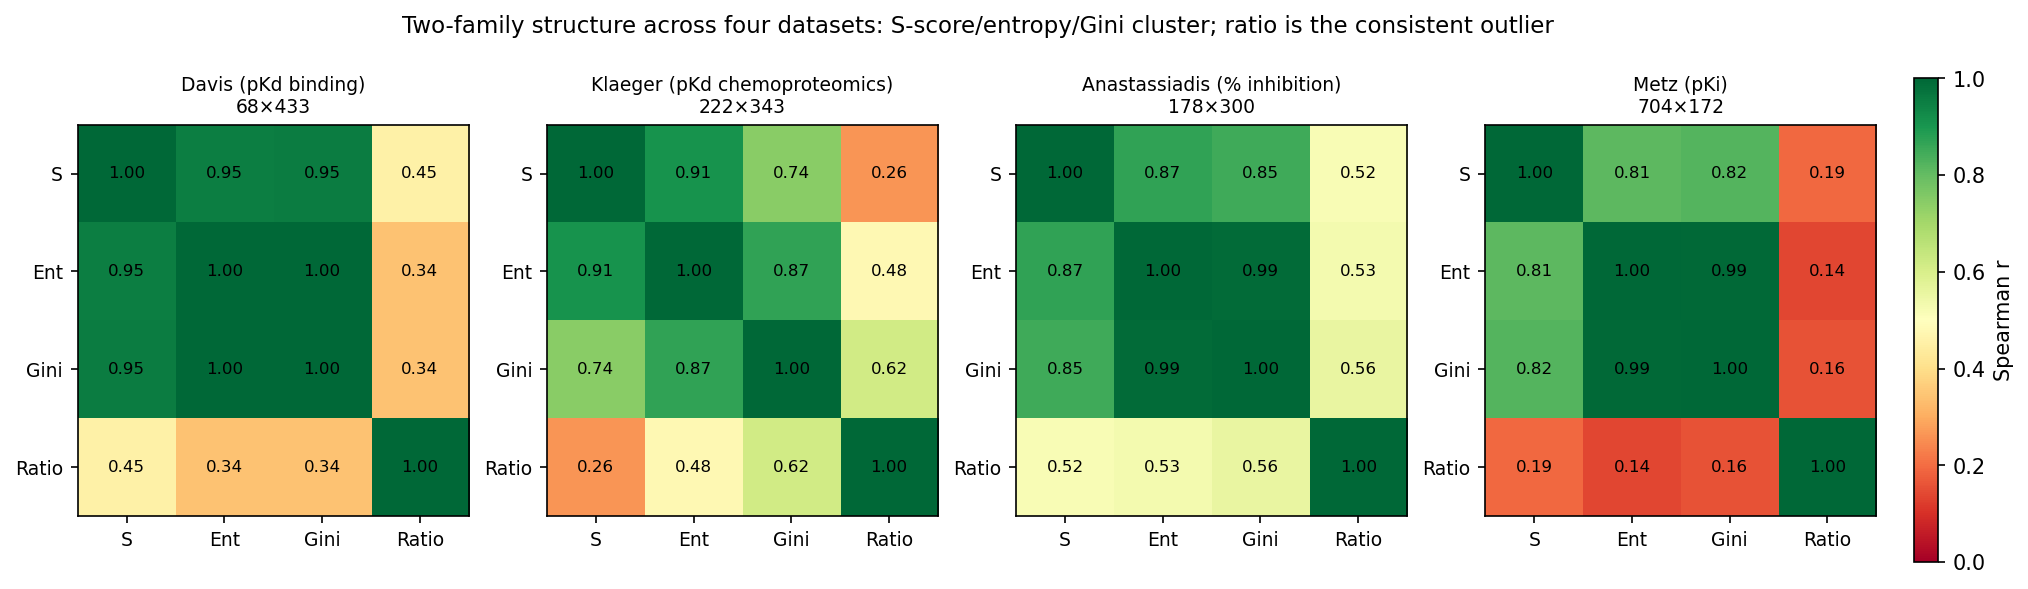
\includegraphics[width=\textwidth]{figures/cross_dataset_correlations}
  \caption{Spearman correlations between the median rankings of the
           four selectivity definitions, computed independently on each of the
           four datasets (compound $\times$ kinase panel sizes shown).
           In every dataset the S-score (S), entropy (Ent), and Gini cluster
           together while the ratio is the consistent outlier (the ratio row
           and column are the least green throughout), confirming the
           two-family structure across competition-binding, chemoproteomic, and
           functional-activity assays.}
  \label{fig:crossdataset}
\end{figure}

\subsection{Rank Instability Is Structured and Predictable}

\begin{figure}[h]
  \centering
  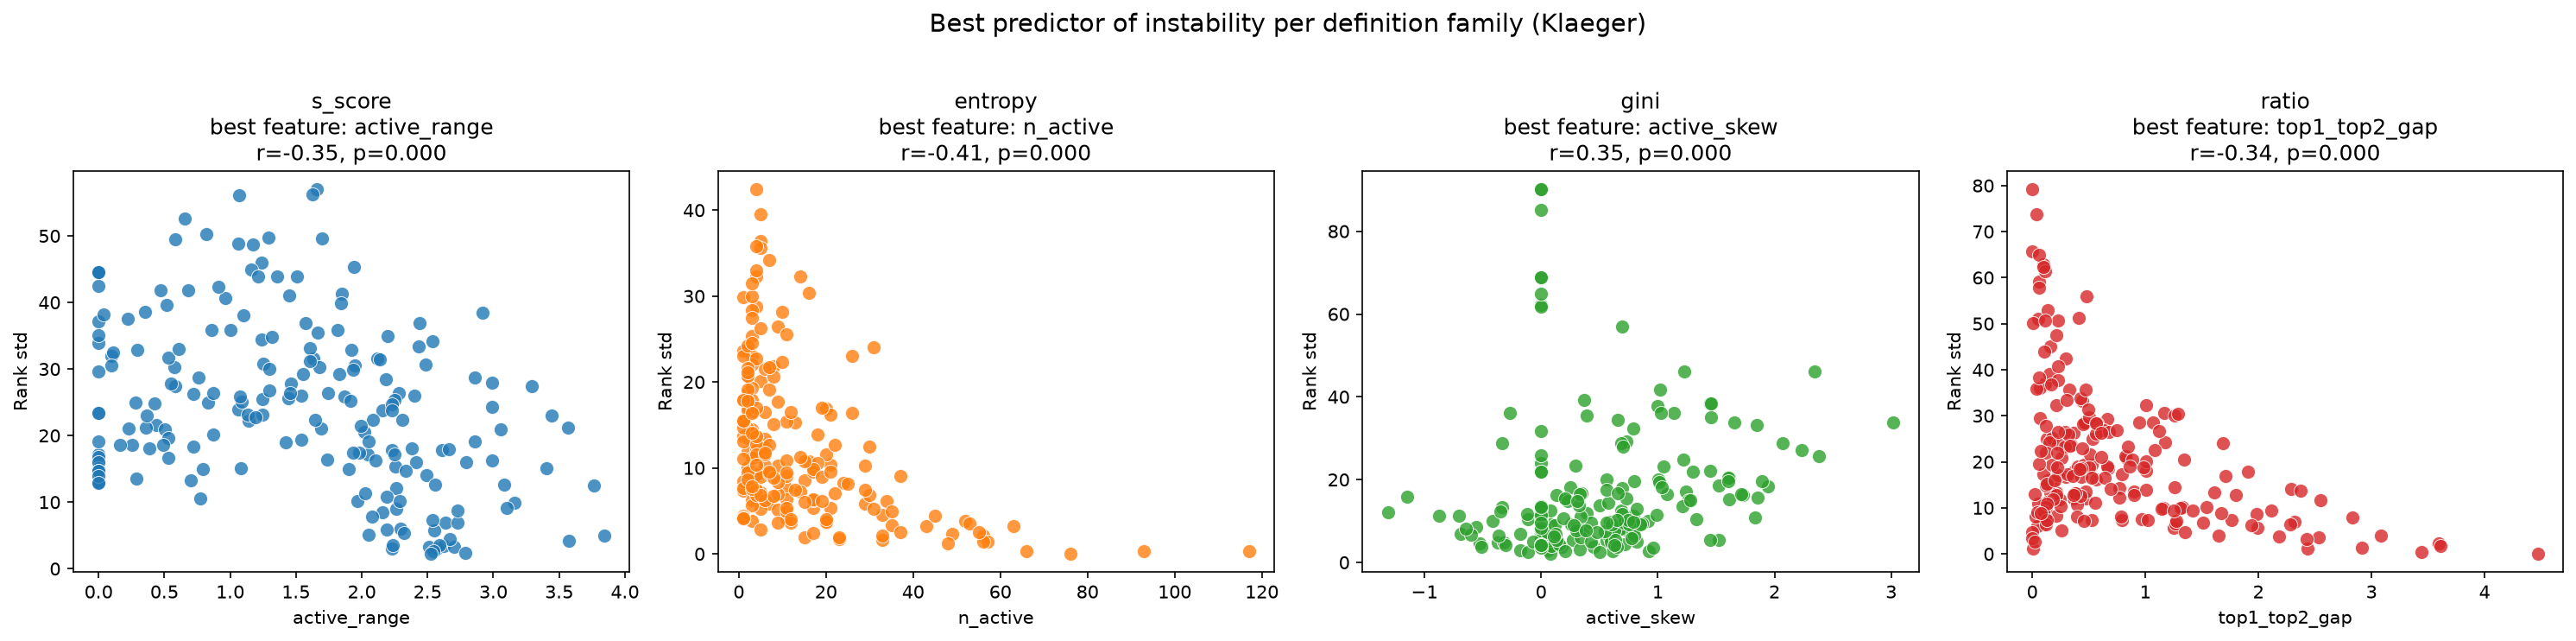
\includegraphics[width=0.85\textwidth]{figures/instability_by_family}
  \caption{Best predictor of rank instability within each definition family
           (Klaeger dataset, active compounds, $n=206$).
           Ratio instability is best predicted by the top$_1$--top$_2$ affinity gap;
           entropy, Gini, and S-score instability are best predicted by features
           of the active affinity distribution.}
  \label{fig:instability}
\end{figure}

\label{sec:results:instability}

Overall rank instability --- measured as the standard deviation of a
compound's rank across all 30 configurations --- varies substantially across
compounds (Klaeger: mean $\sigma = 35.4$, range $7.1$--$91.6$;
Davis: mean $\sigma = 8.5$, range $1.6$--$19.3$).
Instability is not uniformly distributed: within each definition family,
specific binding profile features predict which compounds receive unstable
rankings (Table~\ref{tab:predictors}).

Within the ratio family, the gap between the top and second-ranked affinities
(top$_1$--top$_2$ gap) is the strongest predictor of instability
(Figure~\ref{fig:instability})
($r = -0.446$, $p < 0.001$ on Davis; $r = -0.341$, $p < 0.001$ on Klaeger).
Compounds with near-identical affinities for their two best-bound kinases
receive highly variable ratio rankings because the choice of reference
off-target ($k = 1$ vs.\ $k = 2, \ldots, 5$) determines whether the compound
appears selective or promiscuous.

Within the entropy and Gini families, the number of active kinases
($\mathrm{p}K_d > 6$) negatively predicts instability
($r = -0.279$, $p < 0.05$ for entropy on Davis;
$r = -0.455$, $p < 0.001$ on Klaeger).
Compounds with many active kinases have well-defined broad profiles whose
entropy and Gini scores are stable across baseline choices; compounds with few
active kinases are sensitive to the baseline because small changes can move
targets in or out of the active set, altering the distribution substantially.
The active affinity range is also a significant predictor for the S-score and
entropy on Klaeger ($r = -0.46$ and $-0.32$, both $p < 0.001$; Gini
$r = -0.16$, $p < 0.05$), consistent with the interpretation that heterogeneous
profiles are easier to rank stably than flat ones.

S-score instability is not significantly predicted by any profile feature on
either dataset, suggesting that it is driven primarily by where compounds fall
relative to the threshold rather than by intrinsic profile shape.

\begin{table}[h]
  \centering
  \caption{Spearman correlations between binding profile features and
           within-family rank instability on the Klaeger dataset ($n=206$
           active drugs). Significance: * $p<0.05$, ** $p<0.01$,
           *** $p<0.001$.}
  \label{tab:predictors}
  \begin{tabular}{lcccc}
    \toprule
    Feature & S-score & Entropy & Gini & Ratio \\
    \midrule
    $n_\mathrm{active}$      & $-0.350^{***}$ & $-0.455^{***}$ & $-0.166^{*}$   & $-0.040$ \\
    top$_1$--top$_2$ gap     & $+0.058$       & $+0.128$       & $+0.109$       & $-0.341^{***}$ \\
    Active affinity std      & $-0.386^{***}$ & $-0.215^{**}$  & $-0.176^{*}$   & $-0.107$ \\
    Active affinity range    & $-0.458^{***}$ & $-0.318^{***}$ & $-0.163^{*}$   & $-0.116$ \\
    top$_2$ $\mathrm{p}K_d$  & $-0.394^{***}$ & $-0.282^{***}$ & $-0.268^{***}$ & $+0.186^{**}$ \\
    \bottomrule
  \end{tabular}
\end{table}

\subsection{Three Mechanistically Distinct Sources of Instability}

\begin{figure}[h]
  \centering
  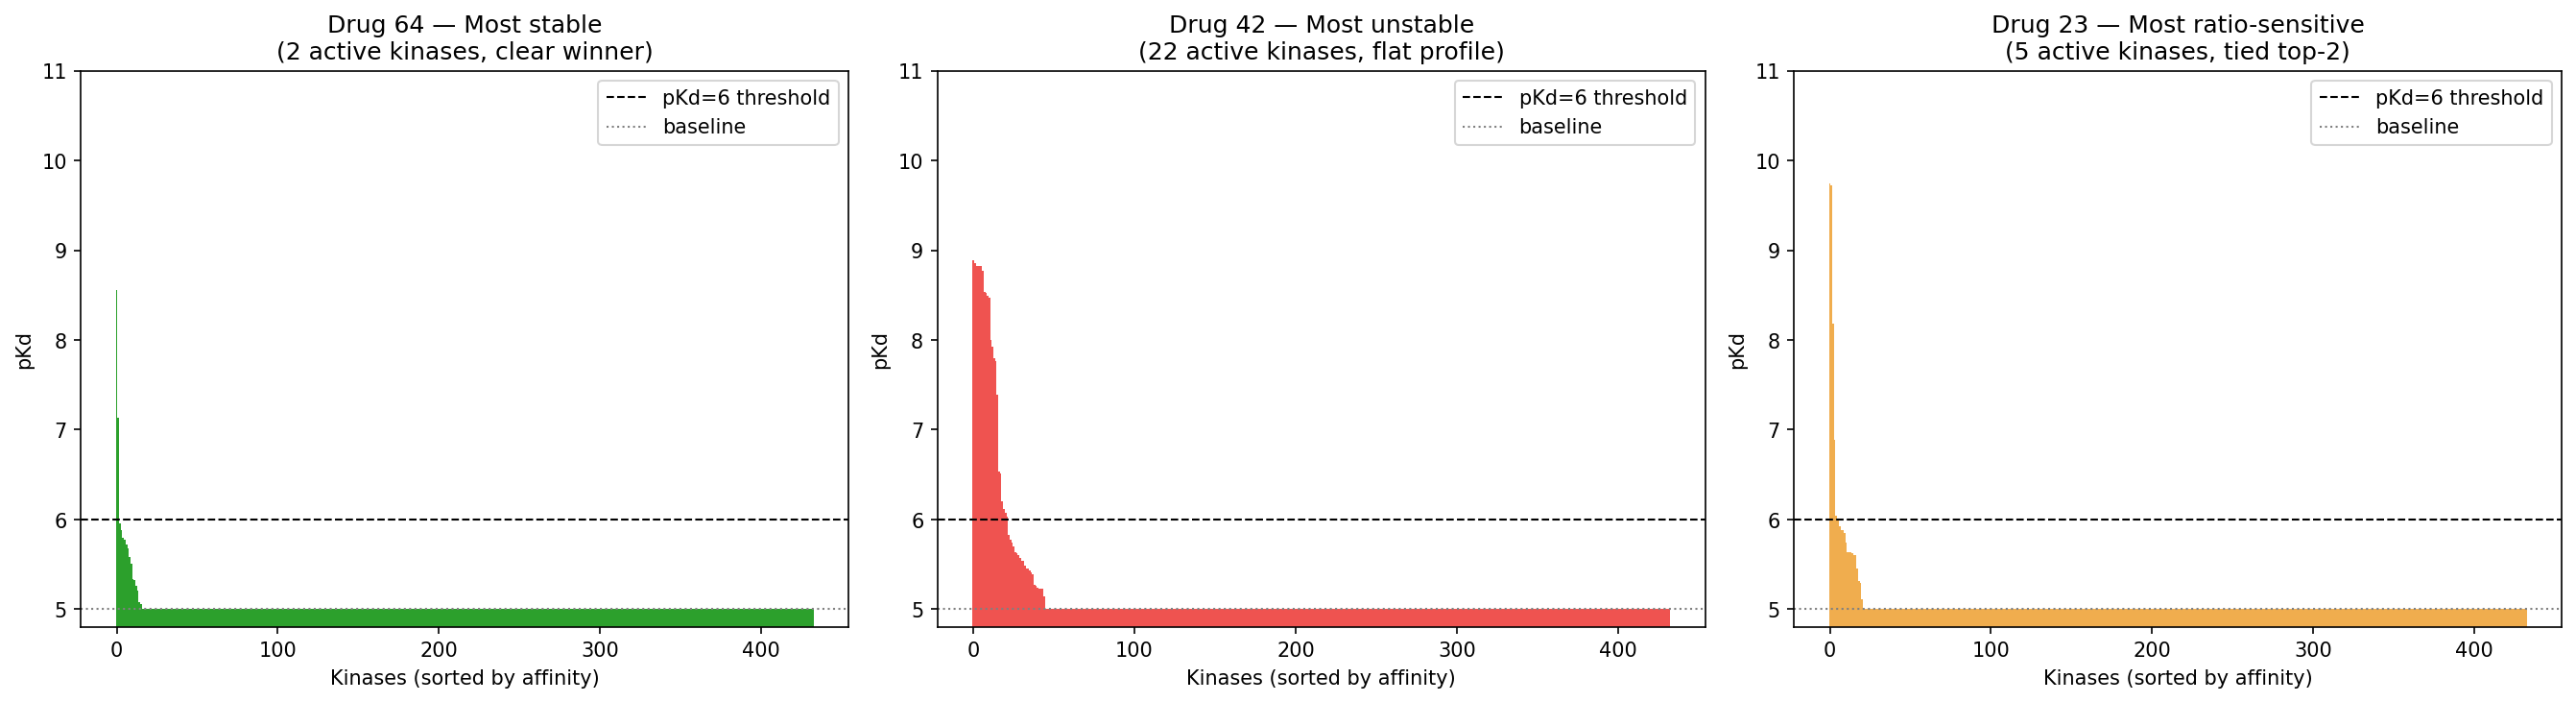
\includegraphics[width=0.85\textwidth]{figures/binding_profiles}
  \caption{Representative binding profiles illustrating the three instability types.
           Left: Drug~64 (Davis), most stable ($\sigma = 1.6$), two active kinases.
           Center: Drug~42 (Davis), most unstable ($\sigma = 19.3$), 22 active kinases
           at near-identical affinities.
           Right: Drug~23 (Davis), most ratio-sensitive, five active kinases
           including two near-tied top targets ($\Delta\mathrm{p}K_d = 0.019$).
           Dashed line: $\mathrm{p}K_d = 6$ activity threshold;
           dotted line: $\mathrm{p}K_d = 5$ assay floor.}
  \label{fig:profiles}
\end{figure}

\label{sec:results:taxonomy}

Examination of the most and least unstable compounds in the Klaeger dataset
reveals three structurally distinct sources of rank instability
(Figure~\ref{fig:profiles}), each
implicating a different aspect of how the definitions are constructed.

\textbf{Type~1 --- Zero-active compounds.}
The five most unstable Klaeger compounds (e.g.\ AZD-8055, BMS-911543,
Filgotinib; rank $\sigma > 80$) all have zero active kinases at the
$\mathrm{p}K_d > 6$ threshold.
These compounds have no meaningful binding to any profiled kinase at
sub-micromolar affinity, yet all four definitions still assign them numerical
selectivity scores based on the detection floor values.
The resulting rankings are arbitrary: different parameterizations produce
different orderings of compounds that are, in practice,
indistinguishable from one another.
Mean rank instability for zero-active compounds is $\sigma \approx 74$,
compared with $\sigma \approx 32$ for compounds with at least one active
kinase ($p < 0.001$, Mann--Whitney $U$ test).
This pattern is observed only in the Klaeger dataset; all Davis compounds
have at least one active kinase, consistent with Davis's fixed-concentration
screening design, which reports a $K_d$ only when activity is first detected
at 10~$\mu$M.

\textbf{Type~2 --- Near-tied top targets.}
Among active compounds, ratio-specific instability is strongly predicted by a
small top$_1$--top$_2$ gap ($r = -0.341$, $p < 0.001$).
Compounds such as Dovitinib (top$_1$--top$_2$ gap $= 1.935$~pKd units) and
BMS-690514 (gap $= 1.985$) show large entropy-ratio disagreement despite
having well-defined primary targets, because the ratio definition is sensitive
to whether the reference off-target is the second or a lower-ranked kinase.
By contrast, Drug~23 in the Davis dataset (top$_1$--top$_2$ gap $= 0.019$)
shows maximal ratio instability because its two best-bound kinases are
essentially indistinguishable, making the ratio highly sensitive to which is
designated the primary target.

\textbf{Type~3 --- Broad profiles with a dominant primary target.}
The largest entropy-ratio disagreements in the Klaeger dataset arise for
compounds with high $n_\mathrm{active}$ and a large top$_1$--top$_2$ gap
(e.g.\ Dovitinib: $n_\mathrm{active} = 26$, gap $= 1.935$;
BMS-690514: $n_\mathrm{active} = 20$, gap $= 1.985$).
These compounds have one clearly dominant target but also bind many kinases at
moderate affinity.
The ratio definition scores them as highly selective (large gap between primary
and secondary target), while the entropy and Gini definitions score them as
moderately promiscuous (activity spread across many targets).
Neither characterization is incorrect; they reflect genuinely different
questions about selectivity.

Conversely, the most stable compounds in both datasets (e.g.\ XL-228,
$\sigma = 7.1$; PF-03814735, $\sigma = 8.1$) are highly promiscuous, with
40--57 active kinases.
When a compound binds nearly the entire profiled kinome, all definitions rank
it as non-selective regardless of parameterization, producing low instability
despite --- or rather because of --- high promiscuity.

\subsection{Panel Size Dependence of Selectivity Rankings}
\label{sec:results:panelsize}

To assess the stability of selectivity rankings as a function of kinase panel
size, we performed a subsampling analysis on the Klaeger dataset.
The Davis dataset was not used for this analysis for two reasons: its complete
matrix design (every compound tested against every kinase by construction)
does not reflect the sparse coverage of real profiling panels, and subsampling
kinases from Davis changes the apparent number of active compounds in ways that
confound the panel size effect with the zero-active instability characterized
in the instability taxonomy above.
The Klaeger dataset, derived from chemoproteomic dose--response profiling with
genuine sparse kinase coverage, is the more appropriate substrate for this
question.
For each panel size $p \in \{50, 80, \ldots, 320, 343\}$, we drew 50 random
subsets of $p$ kinases from the full panel of 343, computed each selectivity
definition on the subpanel, and measured agreement with the full-panel ranking
using Spearman correlation.

The four definitions differ substantially in their panel size requirements
(Figure~\ref{fig:panelsize}).
Selectivity entropy reaches mean $r = 0.90$ against the full-panel ranking at
approximately 110 kinases, and S-score at approximately 140 kinases.
The Gini coefficient requires approximately 290 kinases to reach the same
threshold.
The ratio definition does not reach $r = 0.90$ until the panel contains 320
or more kinases, and achieves $r = 0.888$ even at 320 kinases --- only 23
below the full panel size.

This result has a direct practical implication.
Standard commercial kinase selectivity panels typically profile 50--100
kinases.\cite{Bosc2017}
At these panel sizes, entropy- and S-score-based rankings are reasonably
stable ($r \approx 0.76$--$0.85$), but Gini and ratio rankings are effectively
uncorrelated with what would be obtained on a full kinome panel
($r < 0.14$ for Gini, $r < 0.00$ for ratio at $p = 50$).
Ratio rankings in particular are unreliable at any panel size commonly used
in practice, because the identity of the reference off-target ($k$-th ranked
kinase) changes substantially as panel composition changes.
This is further evidence that ratio-based definitions measure a qualitatively
different property from distribution-based definitions, and reinforces D2
(bounded gap sensitivity) as a necessary property.

\begin{figure}[h]
  \centering
  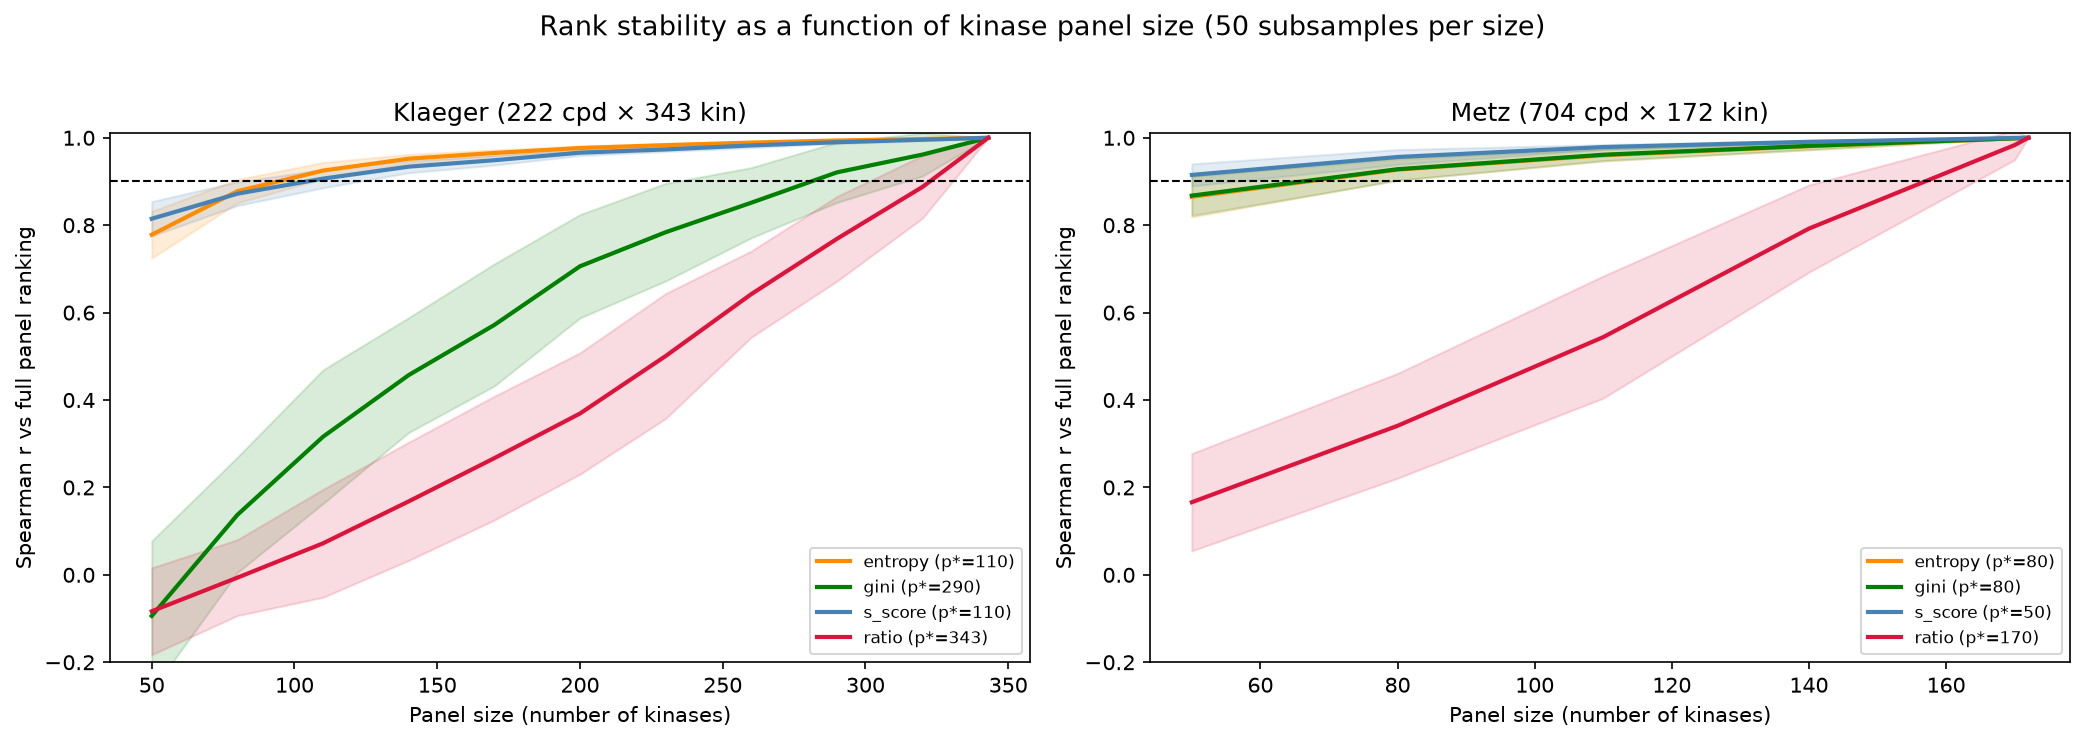
\includegraphics[width=0.75\textwidth]{figures/panel_size_stability}
  \caption{Mean Spearman correlation between rankings computed on random
           kinase subpanels and rankings on the full Klaeger panel (343
           kinases), as a function of subpanel size.
           Shaded bands indicate $\pm 1$ standard deviation across 50
           subsamples.
           The dashed line marks $r = 0.90$.
           Entropy and S-score rankings stabilize at approximately 110--140
           kinases; Gini requires approximately 290 kinases; ratio does not
           reach $r = 0.90$ at any practically used panel size.}
  \label{fig:panelsize}
\end{figure}

\section{Required Properties for a Well-Formed Selectivity Measure}
\label{sec:desiderata}

The empirical findings of the Results section motivate four properties that any
well-formed kinase inhibitor selectivity measure should satisfy.
Each property is stated below together with the observed failure mode that
motivates it.
We call them required properties because they are necessary conditions: a
measure that violates any one of them produces the rank instabilities
documented above.

Let $\mathbf{x} = (x_1, \ldots, x_N) \in \mathbb{R}^N$ denote a compound's
binding profile across $N$ kinases, where $x_i = \mathrm{p}K_{d,i}$.
A selectivity measure is a function $f : \mathbb{R}^N \to \mathbb{R}$, where
higher values indicate greater selectivity.
A selectivity ranking over a set of compounds is induced by ordering their
$f$-scores.

\paragraph{D1 --- Reliability threshold.}
There exists a threshold $\tau^* > 0$ such that $f(\mathbf{x})$ is undefined,
or explicitly flagged as unreliable, when $\max_i x_i \leq \tau^*$.

\textit{Motivation.}
Compounds with no detected binding above the assay detection floor receive
arbitrary selectivity scores under all four definitions studied here, producing
rank instability with mean $\sigma \approx 74$ compared with $\sigma \approx
32$ for active compounds (Type~1 instability, above).
Selectivity is a property of binding; a compound that does not bind cannot be
meaningfully ranked relative to compounds that do.
No existing definition incorporates an explicit reliability condition: both
the S-score and selectivity entropy assign scores to compounds with no
sub-micromolar binding, treating detection floor values as informative.

\paragraph{D2 --- Bounded gap sensitivity.}
For any compound profile $\mathbf{x}$ satisfying D1, a small perturbation to
the identity of the reference off-target should produce a bounded change in
$f(\mathbf{x})$.
Formally, if $f$ depends on the $k$-th ranked affinity $x_{(k)}$, then
$|f(\mathbf{x}; k) - f(\mathbf{x}; k+1)|$ should be bounded by a function of
$x_{(k)} - x_{(k+1)}$.

\textit{Motivation.}
Ratio-based definitions violate this property when $x_{(1)} \approx x_{(2)}$:
a compound with near-identical affinities for its top two kinases receives a
large ratio score when $k=1$ (the gap to the next off-target may be large) but
a near-zero score when $k=2$ (the gap between the tied targets is negligible).
This produces the Type~2 instability identified in
the instability taxonomy above, where top$_1$--top$_2$ gap is the
strongest predictor of ratio instability ($r = -0.341$, $p < 0.001$).
Distribution-based definitions (entropy, Gini) satisfy a weaker version of
this property because they do not privilege any single pairwise comparison.

\paragraph{D3 --- Distributional consistency.}
The ranking induced by $f$ should be stable under small perturbations to the
activity baseline $\beta$ used to define the active binding distribution.
Formally, for any two compounds $\mathbf{x}, \mathbf{y}$ and any
$\epsilon > 0$, there exists $\delta > 0$ such that if $|\beta_1 - \beta_2|
< \delta$ then the ranking of $\mathbf{x}$ relative to $\mathbf{y}$ under
$f(\cdot; \beta_1)$ agrees with that under $f(\cdot; \beta_2)$.

\textit{Motivation.}
The entropy and Gini definitions are parameterized by a baseline $\beta$ that
determines which affinities contribute to the binding distribution.
Compounds with few active kinases are sensitive to this choice because small
changes in $\beta$ can move individual kinases in or out of the active set,
substantially altering the distribution.
The negative correlation between $n_\mathrm{active}$ and entropy/Gini
instability ($r = -0.47$ on Klaeger, $p < 0.001$) reflects this sensitivity.
D3 requires that the ranking be robust to the choice of $\beta$ within a
reasonable neighborhood, which existing implementations do not guarantee.

\paragraph{D4 --- Monotonicity under weak off-target addition.}
If compound $\mathbf{x}$ has a weak additional binding interaction added ---
formally, if $\mathbf{x}' = (x_1, \ldots, x_N, x_{N+1})$ where $x_{N+1} \leq
\tau^*$ --- then $f(\mathbf{x}') \leq f(\mathbf{x})$.
Adding a sub-threshold binding interaction should not increase a compound's
selectivity score.

\textit{Motivation.}
Ratio-based definitions can violate this property: if the new weak interaction
becomes the reference off-target ($k=1$), the ratio to the primary target may
increase, artifactually improving the apparent selectivity score.
This failure mode is practically relevant when profiling panels differ in size
or composition across experiments, as is common when comparing selectivity
across different assay platforms or across datasets such as Davis and Klaeger.
Distribution-based definitions satisfy D4 naturally, since adding a
sub-threshold term to the probability distribution decreases or preserves
entropy and Gini.

\bigskip
Table~\ref{tab:desiderata} summarizes which existing definitions satisfy each
property.
No existing definition satisfies all four simultaneously.
Whether a single measure can satisfy all four at once remains an open question.

\begin{table}[h]
  \centering
  \caption{Satisfaction of the four required properties by existing
           selectivity definitions.
           $\checkmark$: satisfied by construction.
           $\sim$: partially satisfied or satisfied under additional assumptions.
           $\times$: violated in general.}
  \label{tab:desiderata}
  \begin{tabular}{lcccc}
    \toprule
    Property & S-score & Entropy & Gini & Ratio \\
    \midrule
    D1 (reliability threshold)        & $\times$ & $\times$ & $\times$ & $\times$ \\
    D2 (bounded gap sensitivity)      & $\sim$   & $\checkmark$ & $\checkmark$ & $\times$ \\
    D3 (distributional consistency)   & $\sim$   & $\times$ & $\times$ & $\checkmark$ \\
    D4 (monotonicity, weak off-target)& $\checkmark$ & $\checkmark$ & $\checkmark$ & $\times$ \\
    \bottomrule
  \end{tabular}
\end{table}

\section{Discussion}
\label{sec:discussion}

The central finding of this work is that existing kinase inhibitor selectivity
definitions do not measure the same quantity.
The ratio definition and the distribution-based family (S-score, entropy, Gini)
produce substantially different compound rankings (cross-family
$r = 0.14$--$0.62$ across four datasets), and the sources of disagreement are
mechanistically interpretable rather than random.
This has practical consequences: a compound that ratio-based analysis designates
as selective may be designated as moderately promiscuous by entropy-based
analysis, and vice versa, depending on the shape of its binding profile.
Go/no-go decisions in early drug discovery are routinely made on the basis of
selectivity assessments without acknowledgment that the choice of definition
materially affects the outcome.

\subsection{The Two-Family Structure Reflects a Conceptual Distinction}

The clustering of definitions into two families is not a statistical artifact
but reflects a genuine difference in what is being measured.
Distribution-based definitions ask: how concentrated is the compound's binding
activity across the full profiled kinome?
The ratio definition asks: how much more potently does the compound bind its
primary target than a specified off-target?
These are distinct questions with distinct answers for a large class of
compounds --- specifically, those with one clearly dominant target that also
bind many kinases at moderate affinity (Type~3 profiles in our taxonomy).
For such compounds, ratio-based methods report high selectivity while
distribution-based methods report moderate promiscuity, and both
characterizations are correct given their respective questions.

The disagreement is therefore not a defect to be corrected by choosing the
``right'' definition, but a signal that the field has not agreed on what
selectivity means.
The required properties proposed in the Required Properties section are an
attempt to make this question precise enough that it can be answered formally.

\subsection{The Historical Roots of Definitional Ambiguity}

The coexistence of ratio-based and distribution-based selectivity definitions
in the kinase inhibitor literature has a historical explanation rooted in the
structure of the selectivity question itself.
In classical pharmacology and analytical chemistry, selectivity is inherently
pairwise: how much more potently does a compound bind target A than target B?
IUPAC formalizes this for analytical methods as a selectivity coefficient ---
the ratio of binding constants for analyte and interferent --- and organic
chemistry quantifies chemo-, regio-, and stereoselectivity as ratios of
competing rate constants.\cite{IUPAC2001}
These ratio definitions are appropriate because the question is binary.

Kinase inhibitor selectivity, by contrast, is a distributional question: how
concentrated is a compound's binding activity across a panel of hundreds of
kinases?
This is structurally different from a pairwise comparison, and ratio-based
measures are poorly suited to it precisely because they discard all but two
data points from a profile of 300--500 kinases, as the panel size analysis
makes quantitative.
The entropy and Gini definitions were introduced specifically because
researchers recognized that ratio measures were inadequate for large panels,
but the older definitions were never retired.
The result is a field that applies pairwise measures to distributional
questions and distributional measures to pairwise questions, without a
principled basis for choosing between them.
The required properties proposed above can be understood as an attempt
to make this distinction precise: D2 (bounded gap sensitivity) and D4
(monotonicity) are properties that ratio definitions violate specifically
because they treat a distributional problem as pairwise, while D3
(distributional consistency) is a property that ratio definitions satisfy
trivially because they do not use a distributional baseline at all.

\subsection{Practical Recommendations}

Pending a formal resolution, three practical recommendations follow from our
findings.

First, D1 (reliability threshold) should be adopted immediately as a reporting
standard.
Compounds with no detected binding above the assay detection floor should not
receive selectivity scores, or should have their scores explicitly flagged as
unreliable.
Of the 222 Klaeger compounds, 16 (7.2\%) fall into this category and currently
receive scores that are indistinguishable from noise.

Second, selectivity assessments should report the sensitivity of rankings to
parameter choice rather than a single score at a single parameter value.
Our analysis shows that rank standard deviation across the parameter sweep is a
compound-specific, interpretable quantity that identifies which compounds have
robust selectivity assessments and which do not.
This is analogous to reporting confidence intervals in statistical estimation.

Third, when comparing selectivity across studies that use different definitions,
the comparison should be restricted to the subset of compounds and parameter
values for which the definitions agree.
The high within-family correlations ($r > 0.74$) suggest that S-score, entropy,
and Gini are interchangeable for most purposes when parameters are chosen
consistently; ratio-based measures should not be compared directly with
distribution-based measures without acknowledging the conceptual distinction.

\subsection{Limitations}

The analysis covers four profiling datasets spanning three assay technologies
and two readout types, but these still represent a fraction of the chemical and
kinase space relevant to drug discovery.
The assay technologies are not directly comparable in absolute terms --- the
active-compound fractions differ across datasets for both genuine
selectivity reasons and assay-specific detection thresholds --- so our analysis
relies on within-dataset rank comparisons rather than cross-dataset absolute
scores.
The consistency of the two-family structure and the instability predictors
across all four datasets indicates that the findings are not artifacts of a
single assay platform, but findings should still be interpreted in light of
these technological differences.

We also examined whether in vitro selectivity predicts clinical toxicity,
correlating the selectivity rankings of the FDA-approved Klaeger compounds with
FAERS adverse-event rates ($n = 46$) and FDA-label discontinuation rates
($n = 33$).
No association was significant under any definition (all $|r| < 0.27$, all
$p > 0.13$).
We attribute this to confounding --- FAERS counts track prescription volume and
indication prevalence, and label discontinuation rates reflect
indication-specific trial populations --- rather than to a genuine absence of
relationship.
A proper test would require indication-stratified, treatment-related
adverse-event rates from controlled trials with matched comparators, which are
not available in standardized form across these drugs.
Full details are given in the Supporting Information.

The four properties proposed above are necessary
conditions motivated by empirical failure modes; they are not proven to be
sufficient to uniquely characterize a selectivity measure, and it is not known
whether they are jointly satisfiable.
The satisfaction assessments in Table~\ref{tab:desiderata} are based on
analysis of the functional forms of each definition and the empirical findings
of this study; a formal proof of satisfaction or violation for each
property--definition pair is left for future work.

\section{Conclusion}
\label{sec:conclusion}

We have shown that commonly used kinase inhibitor selectivity definitions
cluster into two families that measure fundamentally different properties of
binding profiles, that rank instability within and between families is
mechanistically predictable from binding profile shape, and that three
structurally distinct sources of instability can be identified and
characterized.
These findings motivate four required properties --- a reliability threshold
condition, bounded gap sensitivity, distributional consistency, and monotonicity
under weak off-target addition --- that any well-formed selectivity measure
should satisfy.
No existing definition satisfies all four simultaneously.

The immediate practical implication is that selectivity assessments should
report the sensitivity of rankings to parameter choice, and should explicitly
flag compounds with no binding above the detection threshold as unreliable.
The longer-term implication is that the field needs a principled basis for
choosing among selectivity definitions rather than applying them
interchangeably.
The four required properties proposed here are a concrete starting point: a
well-formed measure should satisfy all of them, and identifying or constructing
such a measure is the natural next step.


\begin{acknowledgement}
The authors thank the developers of the Davis and Klaeger datasets for making
their data publicly available.
The author used Claude (Anthropic, claude.ai), a large language model assistant,
during the preparation of this manuscript.
Specifically, Claude was used to assist with: data analysis code development and
debugging in Python; literature search and identification of related work;
drafting and editing of manuscript text; and research planning and
interpretation of results.
All scientific conclusions, the conceptual framework, the required properties proposed in the
Required Properties section, and the final manuscript content were developed, verified, and
approved by the author.
The author takes full responsibility for the accuracy and integrity of all
content in this work.
The use of Claude does not transfer any rights over the content of this manuscript
to Anthropic or any third party.
\end{acknowledgement}

\begin{suppinfo}
Figure~S1: operationalization-sensitivity check comparing the entropy and Gini
rankings computed in forms close to the original publications
(association-constant weighting) with the baseline-subtracted log-affinity forms
used in the main text.
Clinical outcome analysis: methods and full results of the secondary analysis
relating selectivity rankings to FAERS adverse-event report rates and FDA-label
discontinuation rates for the FDA-approved Klaeger compounds, including the
per-definition correlations and the openFDA queries used.
A preprint of this manuscript is available on ChemRxiv at
\url{https://doi.org/10.26434/chemrxiv.15001618/v1}.
\end{suppinfo}

\section*{Data and Software Availability}
All data and software used in this study are publicly available.
The Davis kinase inhibitor profiling dataset is available at
\url{https://github.com/dingyan20/Davis-Dataset-for-DTA-Prediction}.
The Klaeger et al.\ dataset is available as supplementary data to the
original publication (Science, 2017, \url{https://doi.org/10.1126/science.aan4368}).
The Anastassiadis et al.\ (\emph{Nat. Biotechnol.} 2011) and Metz et al.\
(\emph{Nat. Chem. Biol.} 2011) datasets are available as supplementary data to
their original publications
(\url{https://doi.org/10.1038/nbt.2017}; \url{https://doi.org/10.1038/nchembio.530}).
All analysis scripts, processed data files, and the \LaTeX\ source for
this manuscript are available at
\url{https://github.com/polinavino/kinase-selectivity-definitions}.
No confidential data were used in this study.
All results reported in this manuscript are fully reproducible from the
publicly available data and code.

\bibliography{references}

\end{document}
